% Made up for the tikra benchmark.
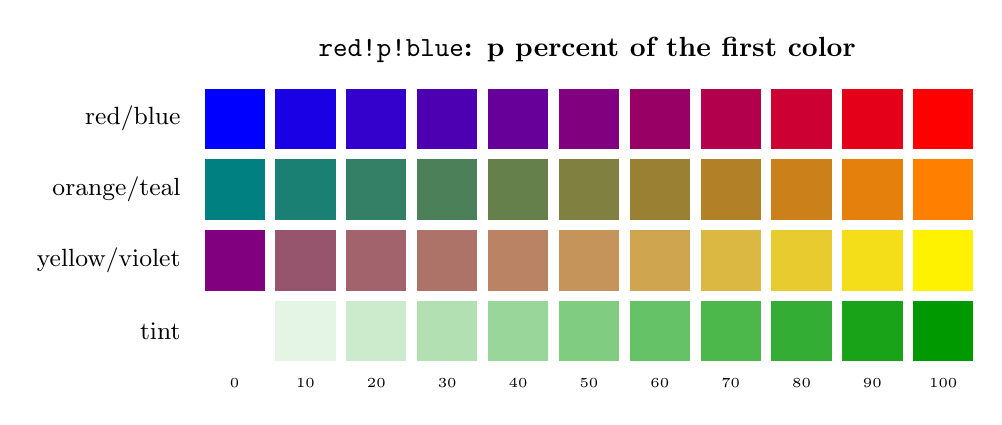
\begin{tikzpicture}[x=0.9cm, y=0.9cm]
  \foreach \p [count=\i from 0] in {0,10,...,100} {
    \fill[red!\p!blue] (\i,0) rectangle +(0.85,0.85);
    \fill[orange!\p!teal] (\i,-1) rectangle +(0.85,0.85);
    \fill[yellow!\p!violet] (\i,-2) rectangle +(0.85,0.85);
    \fill[green!60!black!\p!white] (\i,-3) rectangle +(0.85,0.85);
    \node[font=\tiny, anchor=north] at (\i+0.425,-3.1) {\p};
  }
  \node[anchor=east, font=\small] at (-0.2,0.425) {red/blue};
  \node[anchor=east, font=\small] at (-0.2,-0.575) {orange/teal};
  \node[anchor=east, font=\small] at (-0.2,-1.575) {yellow/violet};
  \node[anchor=east, font=\small] at (-0.2,-2.575) {tint};
  \node[font=\bfseries] at (5.4,1.4) {\texttt{red!p!blue}: p percent of the first color};
\end{tikzpicture}
